\documentclass[twoside]{book}

% Packages required by doxygen
\usepackage{calc}
\usepackage{doxygen}
\usepackage{graphicx}
\usepackage[utf8]{inputenc}
\usepackage{makeidx}
\usepackage{multicol}
\usepackage{multirow}
\usepackage{textcomp}
\usepackage[table]{xcolor}

% Font selection
\usepackage[T1]{fontenc}
\usepackage{mathptmx}
\usepackage[scaled=.90]{helvet}
\usepackage{courier}
\usepackage{amssymb}
\usepackage{sectsty}
\renewcommand{\familydefault}{\sfdefault}
\allsectionsfont{%
  \fontseries{bc}\selectfont%
  \color{darkgray}%
}
\renewcommand{\DoxyLabelFont}{%
  \fontseries{bc}\selectfont%
  \color{darkgray}%
}

% Page & text layout
\usepackage{geometry}
\geometry{%
  a4paper,%
  top=2.5cm,%
  bottom=2.5cm,%
  left=2.5cm,%
  right=2.5cm%
}
\tolerance=750
\hfuzz=15pt
\hbadness=750
\setlength{\emergencystretch}{15pt}
\setlength{\parindent}{0cm}
\setlength{\parskip}{0.2cm}
\makeatletter
\renewcommand{\paragraph}{%
  \@startsection{paragraph}{4}{0ex}{-1.0ex}{1.0ex}{%
    \normalfont\normalsize\bfseries\SS@parafont%
  }%
}
\renewcommand{\subparagraph}{%
  \@startsection{subparagraph}{5}{0ex}{-1.0ex}{1.0ex}{%
    \normalfont\normalsize\bfseries\SS@subparafont%
  }%
}
\makeatother

% Headers & footers
\usepackage{fancyhdr}
\pagestyle{fancyplain}
\fancyhead[LE]{\fancyplain{}{\bfseries\thepage}}
\fancyhead[CE]{\fancyplain{}{}}
\fancyhead[RE]{\fancyplain{}{\bfseries\leftmark}}
\fancyhead[LO]{\fancyplain{}{\bfseries\rightmark}}
\fancyhead[CO]{\fancyplain{}{}}
\fancyhead[RO]{\fancyplain{}{\bfseries\thepage}}
\fancyfoot[LE]{\fancyplain{}{}}
\fancyfoot[CE]{\fancyplain{}{}}
\fancyfoot[RE]{\fancyplain{}{\bfseries\scriptsize Generated on Mon Jun 23 2014 11\-:46\-:07 for G\-H\-O\-S\-T by Doxygen }}
\fancyfoot[LO]{\fancyplain{}{\bfseries\scriptsize Generated on Mon Jun 23 2014 11\-:46\-:07 for G\-H\-O\-S\-T by Doxygen }}
\fancyfoot[CO]{\fancyplain{}{}}
\fancyfoot[RO]{\fancyplain{}{}}
\renewcommand{\footrulewidth}{0.4pt}
\renewcommand{\chaptermark}[1]{%
  \markboth{#1}{}%
}
\renewcommand{\sectionmark}[1]{%
  \markright{\thesection\ #1}%
}

% Indices & bibliography
\usepackage{natbib}
\usepackage[titles]{tocloft}
\setcounter{tocdepth}{3}
\setcounter{secnumdepth}{5}
\makeindex

% Hyperlinks (required, but should be loaded last)
\usepackage{ifpdf}
\ifpdf
  \usepackage[pdftex,pagebackref=true]{hyperref}
\else
  \usepackage[ps2pdf,pagebackref=true]{hyperref}
\fi
\hypersetup{%
  colorlinks=true,%
  linkcolor=blue,%
  citecolor=blue,%
  unicode%
}

% Custom commands
\newcommand{\clearemptydoublepage}{%
  \newpage{\pagestyle{empty}\cleardoublepage}%
}


%===== C O N T E N T S =====

\begin{document}

% Titlepage & ToC
\hypersetup{pageanchor=false}
\pagenumbering{roman}
\begin{titlepage}
\vspace*{7cm}
\begin{center}%
{\Large G\-H\-O\-S\-T }\\
\vspace*{1cm}
{\large Generated by Doxygen 1.8.6}\\
\vspace*{0.5cm}
{\small Mon Jun 23 2014 11:46:07}\\
\end{center}
\end{titlepage}
\clearemptydoublepage
\tableofcontents
\clearemptydoublepage
\pagenumbering{arabic}
\hypersetup{pageanchor=true}

%--- Begin generated contents ---
\chapter{G\-H\-O\-S\-T}
\label{index}\hypertarget{index}{}G\-H\-O\-S\-T documentation \begin{DoxyAuthor}{Author}
Florian Richoux
\end{DoxyAuthor}
\section*{Introduction }

G\-H\-O\-S\-T (General meta-\/\-Heuristic Optimization Solving Tool) is a C++11 library designed for Star\-Craft\-: Brood war. G\-H\-O\-S\-T implements a meta-\/heuristic solver aiming to solve any kind of combinatorial and optimization R\-T\-S-\/related problems represented by a C\-S\-P. It is an generalization of the Wall-\/in project (see \href{https://github.com/richoux/Wall-in}{\tt github.\-com/richoux/\-Wall-\/in}).

The source code is available at \href{https://github.com/richoux/GHOST}{\tt github.\-com/richoux/\-G\-H\-O\-S\-T}, and the documentation pages at \href{http://richoux.github.io/GHOST}{\tt richoux.\-github.\-io/\-G\-H\-O\-S\-T}. G\-H\-O\-S\-T is under the terms of the G\-N\-U G\-P\-L v3 licence.

\subsection*{Scientific papers\-: }


\begin{DoxyItemize}
\item Florian Richoux, Jean-\/\-François Baffier and Alberto Uriarte, G\-H\-O\-S\-T\-: A Combinatorial Optimization Solver for R\-T\-S-\/related Problems (to appear).
\item Florian Richoux, Alberto Uriarte and Santiago Ontañón, Walling in Strategy Games via Constraint Optimization (to appear in A\-I\-I\-D\-E 2014 proceedings).
\item Santiago Ontañón, Gabriel Synnaeve, Alberto Uriarte, Florian Richoux, David Churchill and Mike Preuss, \href{http://pagesperso.lina.univ-nantes.fr/~richoux-f/publications/tciaig13.pdf}{\tt A Survey of Real-\/\-Time Strategy Game A\-I Research and Competition in Star\-Craft}, Transactions on Computational Intelligence and A\-I in Games, I\-E\-E\-E, 2013.
\end{DoxyItemize}

\section*{A short C\-S\-P/\-C\-O\-P tutorial }

T\-O\-D\-O

\section*{How to use G\-H\-O\-S\-T? }

T\-O\-D\-O

\section*{How to define and solve my own C\-S\-P problem with G\-H\-O\-S\-T? }

T\-O\-D\-O 
\chapter{Class Index}
\section{Class List}
Here are the classes, structs, unions and interfaces with brief descriptions\+:\begin{DoxyCompactList}
\item\contentsline{section}{\hyperlink{classghost_1_1Constraint}{ghost\+::\+Constraint$<$ Type\+Variable $>$} \\*\hyperlink{classghost_1_1Constraint}{Constraint} is the class encoding constraints of your C\+S\+P/\+C\+OP }{\pageref{classghost_1_1Constraint}}{}
\item\contentsline{section}{\hyperlink{classghost_1_1Domain}{ghost\+::\+Domain} \\*\hyperlink{classghost_1_1Domain}{Domain} is the class encoding the domain of your C\+S\+P/\+C\+OP }{\pageref{classghost_1_1Domain}}{}
\item\contentsline{section}{\hyperlink{structghost_1_1indexException}{ghost\+::index\+Exception} }{\pageref{structghost_1_1indexException}}{}
\item\contentsline{section}{\hyperlink{classghost_1_1NullObjective}{ghost\+::\+Null\+Objective$<$ Type\+Variable $>$} \\*\hyperlink{classghost_1_1NullObjective}{Null\+Objective} is used when no objective functions have been given to the solver (ie, for pure satisfaction runs) }{\pageref{classghost_1_1NullObjective}}{}
\item\contentsline{section}{\hyperlink{classghost_1_1Objective}{ghost\+::\+Objective$<$ Type\+Variable $>$} \\*\hyperlink{classghost_1_1Objective}{Objective} is the class encoding objective functions of your C\+S\+P/\+C\+OP }{\pageref{classghost_1_1Objective}}{}
\item\contentsline{section}{\hyperlink{classghost_1_1Random}{ghost\+::\+Random} }{\pageref{classghost_1_1Random}}{}
\item\contentsline{section}{\hyperlink{classghost_1_1Solver}{ghost\+::\+Solver$<$ Type\+Variable, Type\+Constraint $>$} \\*\hyperlink{classghost_1_1Solver}{Solver} is the class coding the solver itself }{\pageref{classghost_1_1Solver}}{}
\item\contentsline{section}{\hyperlink{structghost_1_1valueException}{ghost\+::value\+Exception} }{\pageref{structghost_1_1valueException}}{}
\item\contentsline{section}{\hyperlink{classghost_1_1Variable}{ghost\+::\+Variable} \\*\hyperlink{classghost_1_1Variable}{Variable} is the class encoding the variables of your C\+S\+P/\+C\+OP }{\pageref{classghost_1_1Variable}}{}
\end{DoxyCompactList}

\chapter{Class Documentation}
\hypertarget{classghost_1_1Solver}{}\section{ghost\+:\+:Solver$<$ Type\+Variable, Type\+Constraint $>$ Class Template Reference}
\label{classghost_1_1Solver}\index{ghost\+::\+Solver$<$ Type\+Variable, Type\+Constraint $>$@{ghost\+::\+Solver$<$ Type\+Variable, Type\+Constraint $>$}}


\hyperlink{classghost_1_1Solver}{Solver} is the class coding the solver itself.  




{\ttfamily \#include $<$solver.\+hpp$>$}



Collaboration diagram for ghost\+:\+:Solver$<$ Type\+Variable, Type\+Constraint $>$\+:\nopagebreak
\begin{figure}[H]
\begin{center}
\leavevmode
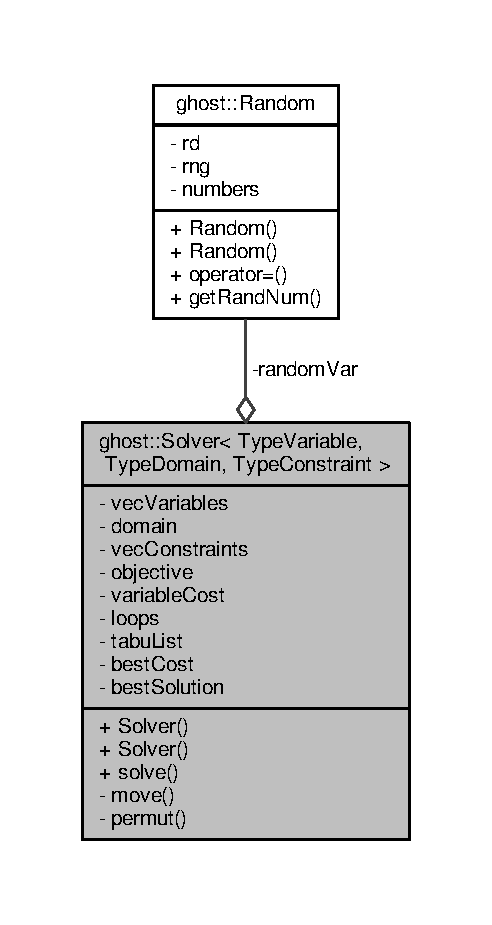
\includegraphics[width=223pt]{classghost_1_1Solver__coll__graph}
\end{center}
\end{figure}
\subsection*{Public Member Functions}
\begin{DoxyCompactItemize}
\item 
\hyperlink{classghost_1_1Solver_afcafbb540e963da0aa0d8bbf5634f6e4}{Solver} (vector$<$ Type\+Variable $>$ \&vec\+Variables, vector$<$ shared\+\_\+ptr$<$ Type\+Constraint $>$$>$ \&vec\+Constraints, shared\+\_\+ptr$<$ \hyperlink{classghost_1_1Objective}{Objective}$<$ Type\+Variable $>$$>$ objecive, bool permutation\+Problem=false)
\begin{DoxyCompactList}\small\item\em \hyperlink{classghost_1_1Solver}{Solver}\textquotesingle{}s regular constructor. \end{DoxyCompactList}\item 
\hyperlink{classghost_1_1Solver_a26fe2a7362fdc6cc44b07e0c658250de}{Solver} (vector$<$ Type\+Variable $>$ \&vec\+Variables, vector$<$ shared\+\_\+ptr$<$ Type\+Constraint $>$$>$ \&vec\+Constraints, bool permutation\+Problem=false)
\begin{DoxyCompactList}\small\item\em Second \hyperlink{classghost_1_1Solver}{Solver}\textquotesingle{}s constructor. \end{DoxyCompactList}\item 
bool \hyperlink{classghost_1_1Solver_ab2f3b79560cefbe8299583a40edad40e}{solve} (double \&final\+Cost, vector$<$ int $>$ \&final\+Solution, double sat\+\_\+timeout, double opt\+\_\+timeout=0.)
\begin{DoxyCompactList}\small\item\em \hyperlink{classghost_1_1Solver}{Solver}\textquotesingle{}s main function, to solve the given C\+S\+P/\+C\+OP. \end{DoxyCompactList}\end{DoxyCompactItemize}


\subsection{Detailed Description}
\subsubsection*{template$<$typename Type\+Variable, typename Type\+Constraint$>$\\*
class ghost\+::\+Solver$<$ Type\+Variable, Type\+Constraint $>$}

\hyperlink{classghost_1_1Solver}{Solver} is the class coding the solver itself. 

You just need to instanciate one \hyperlink{classghost_1_1Solver}{Solver} object, then run its \textquotesingle{}solve\textquotesingle{} function.

The \hyperlink{classghost_1_1Solver}{Solver} class is a template class, waiting for both the type of variable and the type of constraint. Thus, you must instanciate a solver by specifying the class of your variable objects and the class of your constraint objects, like for instance \hyperlink{classghost_1_1Solver}{Solver}$<$My\+Custom\+Variable, My\+Custom\+Constraint$>$ where My\+Custom\+Variable must inherits from \hyperlink{classghost_1_1Variable}{ghost\+::\+Variable} and My\+Custom\+Constraint must inherits from \hyperlink{classghost_1_1Constraint}{ghost\+::\+Constraint}.

Each variable modelling a problem must instanciate the same class. However, constraints of different type can exist within the same problem model. This is the reson why the vector of constraints is a vector of (shared) pointers of \hyperlink{classghost_1_1Constraint}{Constraint}.

\hyperlink{classghost_1_1Solver}{Solver}\textquotesingle{}s constructor also need a shared pointer of an \hyperlink{classghost_1_1Objective}{Objective} object. The reason why \hyperlink{classghost_1_1Objective}{Objective} is not a template parameter of \hyperlink{classghost_1_1Solver}{Solver} but a pointer is to allow a dynamic modification of the objective function.

\begin{DoxySeeAlso}{See also}
\hyperlink{classghost_1_1Variable}{Variable}, \hyperlink{classghost_1_1Constraint}{Constraint}, \hyperlink{classghost_1_1Objective}{Objective} 
\end{DoxySeeAlso}


\subsection{Constructor \& Destructor Documentation}
\index{ghost\+::\+Solver@{ghost\+::\+Solver}!Solver@{Solver}}
\index{Solver@{Solver}!ghost\+::\+Solver@{ghost\+::\+Solver}}
\subsubsection[{\texorpdfstring{Solver(vector$<$ Type\+Variable $>$ \&vec\+Variables, vector$<$ shared\+\_\+ptr$<$ Type\+Constraint $>$$>$ \&vec\+Constraints, shared\+\_\+ptr$<$ Objective$<$ Type\+Variable $>$$>$ objecive, bool permutation\+Problem=false)}{Solver(vector< TypeVariable > &vecVariables, vector< shared_ptr< TypeConstraint >> &vecConstraints, shared_ptr< Objective< TypeVariable >> objecive, bool permutationProblem=false)}}]{\setlength{\rightskip}{0pt plus 5cm}template$<$typename Type\+Variable , typename Type\+Constraint $>$ {\bf ghost\+::\+Solver}$<$ Type\+Variable, Type\+Constraint $>$\+::{\bf Solver} (
\begin{DoxyParamCaption}
\item[{vector$<$ Type\+Variable $>$ \&}]{vec\+Variables, }
\item[{vector$<$ shared\+\_\+ptr$<$ Type\+Constraint $>$$>$ \&}]{vec\+Constraints, }
\item[{shared\+\_\+ptr$<$ {\bf Objective}$<$ Type\+Variable $>$$>$}]{objecive, }
\item[{bool}]{permutation\+Problem = {\ttfamily false}}
\end{DoxyParamCaption}
)}\hypertarget{classghost_1_1Solver_afcafbb540e963da0aa0d8bbf5634f6e4}{}\label{classghost_1_1Solver_afcafbb540e963da0aa0d8bbf5634f6e4}


\hyperlink{classghost_1_1Solver}{Solver}\textquotesingle{}s regular constructor. 


\begin{DoxyParams}{Parameters}
{\em vec\+Variables} & A pointer to the vector of Variables. \\
\hline
{\em vec\+Constraints} & A reference to the vector of Constraints. \\
\hline
{\em obj} & A shared pointer to the \hyperlink{classghost_1_1Objective}{Objective}. \\
\hline
{\em permutation\+Problem} & A boolean indicating if we work on a permutation problem. False by default. \\
\hline
\end{DoxyParams}
\index{ghost\+::\+Solver@{ghost\+::\+Solver}!Solver@{Solver}}
\index{Solver@{Solver}!ghost\+::\+Solver@{ghost\+::\+Solver}}
\subsubsection[{\texorpdfstring{Solver(vector$<$ Type\+Variable $>$ \&vec\+Variables, vector$<$ shared\+\_\+ptr$<$ Type\+Constraint $>$$>$ \&vec\+Constraints, bool permutation\+Problem=false)}{Solver(vector< TypeVariable > &vecVariables, vector< shared_ptr< TypeConstraint >> &vecConstraints, bool permutationProblem=false)}}]{\setlength{\rightskip}{0pt plus 5cm}template$<$typename Type\+Variable , typename Type\+Constraint $>$ {\bf ghost\+::\+Solver}$<$ Type\+Variable, Type\+Constraint $>$\+::{\bf Solver} (
\begin{DoxyParamCaption}
\item[{vector$<$ Type\+Variable $>$ \&}]{vec\+Variables, }
\item[{vector$<$ shared\+\_\+ptr$<$ Type\+Constraint $>$$>$ \&}]{vec\+Constraints, }
\item[{bool}]{permutation\+Problem = {\ttfamily false}}
\end{DoxyParamCaption}
)}\hypertarget{classghost_1_1Solver_a26fe2a7362fdc6cc44b07e0c658250de}{}\label{classghost_1_1Solver_a26fe2a7362fdc6cc44b07e0c658250de}


Second \hyperlink{classghost_1_1Solver}{Solver}\textquotesingle{}s constructor. 


\begin{DoxyParams}{Parameters}
{\em vec\+Variables} & A reference to the vector of Variables. \\
\hline
{\em vec\+Constraints} & A reference to the vector of Constraints. \\
\hline
{\em permutation\+Problem} & A boolean indicating if we work on a permutation problem. False by default. \\
\hline
\end{DoxyParams}


\subsection{Member Function Documentation}
\index{ghost\+::\+Solver@{ghost\+::\+Solver}!solve@{solve}}
\index{solve@{solve}!ghost\+::\+Solver@{ghost\+::\+Solver}}
\subsubsection[{\texorpdfstring{solve(double \&final\+Cost, vector$<$ int $>$ \&final\+Solution, double sat\+\_\+timeout, double opt\+\_\+timeout=0.)}{solve(double &finalCost, vector< int > &finalSolution, double sat_timeout, double opt_timeout=0.)}}]{\setlength{\rightskip}{0pt plus 5cm}template$<$typename Type\+Variable , typename Type\+Constraint $>$ bool {\bf ghost\+::\+Solver}$<$ Type\+Variable, Type\+Constraint $>$\+::solve (
\begin{DoxyParamCaption}
\item[{double \&}]{final\+Cost, }
\item[{vector$<$ int $>$ \&}]{final\+Solution, }
\item[{double}]{sat\+\_\+timeout, }
\item[{double}]{opt\+\_\+timeout = {\ttfamily 0.}}
\end{DoxyParamCaption}
)}\hypertarget{classghost_1_1Solver_ab2f3b79560cefbe8299583a40edad40e}{}\label{classghost_1_1Solver_ab2f3b79560cefbe8299583a40edad40e}


\hyperlink{classghost_1_1Solver}{Solver}\textquotesingle{}s main function, to solve the given C\+S\+P/\+C\+OP. 


\begin{DoxyParams}{Parameters}
{\em final\+Cost} & A reference to the double of the sum of constraints cost for satisfaction problems, or the value of the objective function for optimization problems. For satisfaction problems, a cost of zero means a solution has been found. \\
\hline
{\em final\+Solution} & The configuration of the best solution found, ie, a reference to the vector of assignements of each variable. \\
\hline
{\em sat\+\_\+timeout} & The satisfaction timeout in milliseconds. \\
\hline
{\em opt\+\_\+timeout} & The optimization timeout in milliseconds (optionnal, equals to 10 times sat\+\_\+timeout is not set). \\
\hline
\end{DoxyParams}
\begin{DoxyReturn}{Returns}
True iff a solution has been found. 
\end{DoxyReturn}


The documentation for this class was generated from the following file\+:\begin{DoxyCompactItemize}
\item 
include/\hyperlink{solver_8hpp}{solver.\+hpp}\end{DoxyCompactItemize}

%--- End generated contents ---

% Index
\newpage
\phantomsection
\addcontentsline{toc}{chapter}{Index}
\printindex

\end{document}
